\section{Results}

\subsection{1-D model}

\begin{figure}[here]
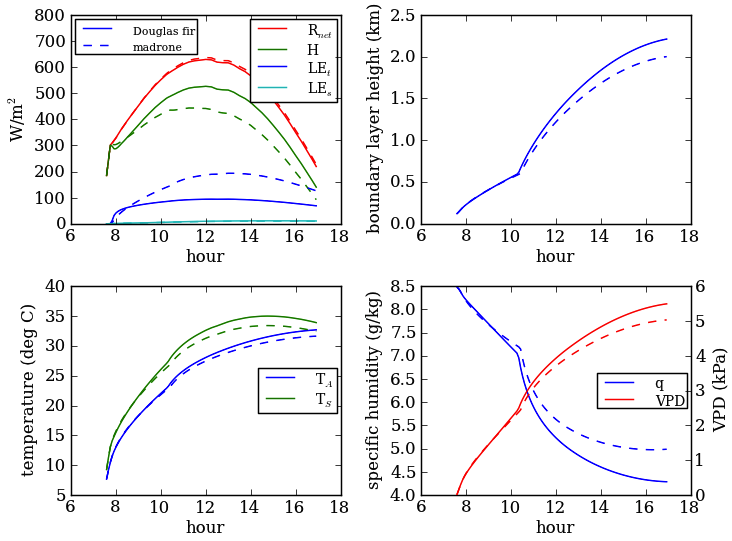
\includegraphics[width=0.9\textwidth]{ch2-BL/figures/testall_Aug15_soilm0pt25_ra10_lapseT2_cropped.png}
\caption{Diurnal cycle simulated by 1-D model for $\theta_{rel}=0.25$ and lapse rate \#2.  Solid lines: Douglas fir case; dashed lines: Pacific madrone case.  Top left: surface energy flux terms ($R_{net}$ is net radiation, $H$ is sensible heat, $LE_t$ is latent heat due to transpiration, and $LE_s$ is latent heat due to soil evaporation.)  Top right: boundary layer height.  Bottom left: surface temperature ($T_S$) and mixed layer air temperature ($T_A$) adjusted to 400 m ASL (ground level in ACRR).  Bottom right: mixed layer specific humidity ($q$) and $VPD$.}
\label{fig:BL_1Ddiurnal}
\end{figure}

The 1-D model simulates a reasonable diurnal cycle for mid-August, but with temperatures several degrees higher than observations at the ACRR, which may result from using tropospheric soundings from Oakland.  Figure \ref{fig:BL_1Ddiurnal} shows a typical diurnal cycle for a moderate lapse rate (\#2) and relative soil moisture $\theta_{rel} = 0.25$.  The Pacific madrone forest has higher transpiration than the Douglas fir forest, because Pacific madrone stomatal conductance is higher at this value of $\theta_{rel}$ (c.f. Figure \ref{fig:BL_FeddesParams}); both cases have very little soil evaporation at this value of $\theta_{rel}$.  As a result, the Pacific madrone case has lower sensible heat ($H$) than the Douglas fir case, leading to a shallower, cooler, and moister boundary layer over the Pacific madrone forest.

\begin{figure}[here]
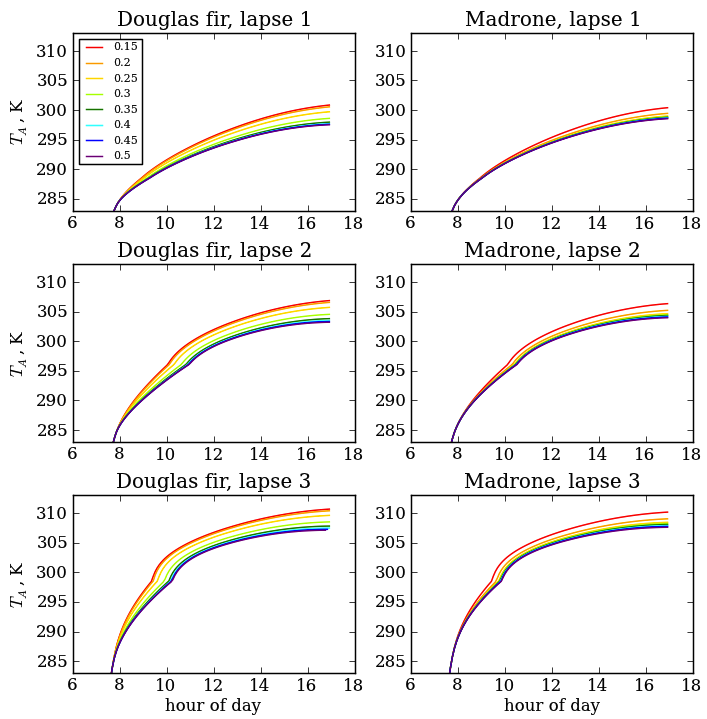
\includegraphics[width=0.9\textwidth]{ch2-BL/figures/testall_compare_sm_lapse_Ta_cropped.png}
\caption{Diurnal cycle of air temperature at 400 m ASL (ground level in ACRR), simulated by the 1-D model, for a range of $\theta_{rel}$ (colors) and free troposphere conditions.  Left column: Douglas fir case; right column: Pacific madrone case.  Top row: lapse rate 1 (coolest free troposphere conditions); middle row: lapse rate 2 (moderate free troposphere conditions); bottom row: lapse rate 3 (warmest free troposphere conditions).}
\label{fig:BL_1DdiurnalTa}
\end{figure}

\begin{figure}[here]
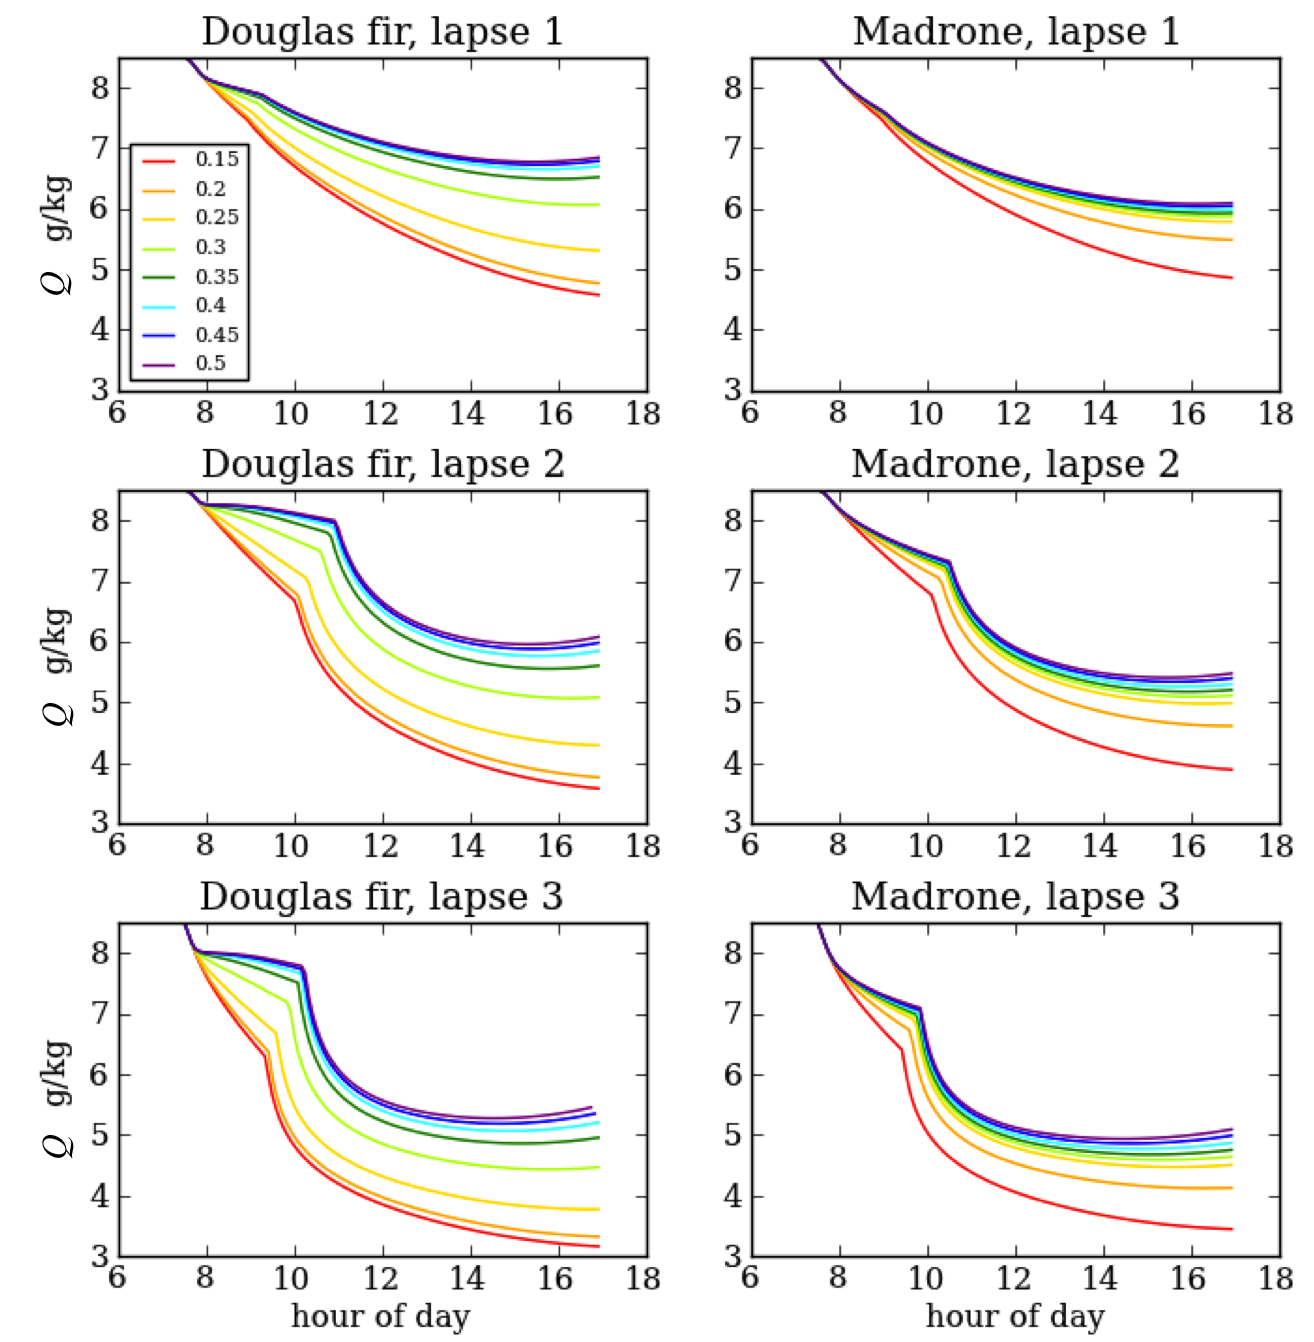
\includegraphics[width=0.9\textwidth]{ch2-BL/figures/testall_compare_sm_lapse_Q_cropped2.png}
\caption{Diurnal cycle of boundary layer specific humidity, simulated by the 1-D model, for a range of $\theta_{rel}$ (colors) and free troposphere conditions.  Left column: Douglas fir case; right column: Pacific madrone case.  Top row: lapse rate 1 (most moist free troposphere conditions); middle row: lapse rate 2 (moderate free troposphere conditions); bottom row: lapse rate 3 (driest free troposphere conditions).}
\label{fig:BL_1DdiurnalQ}
\end{figure}

%\clearpage

The boundary layer is warmer and drier when the free troposphere is warmer and drier (Figures \ref{fig:BL_1DdiurnalTa} and \ref{fig:BL_1DdiurnalQ}; increasing $T_a$ and decreasing $Q$ from lapse rate 1 to 2 to 3).  Additionally, the shape of the diurnal cycle differs among the free troposphere cases, with most rapid morning increase in $T_a$ in the hottest case (lapse rate 3), due to entrainment of high-$\Theta$ air in the steep low-level inversion.  The drier free troposphere conditions in lapse rate 3 also lead to lower $Q$, but with a slower morning decline of $Q$ because of relatively slow boundary layer growth through the steep inversion.

\begin{figure}[here]
\begin{subfigure}{0.5\textwidth}
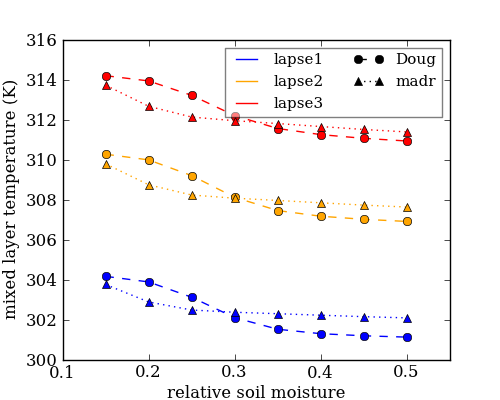
\includegraphics[width=\textwidth]{ch2-BL/figures/all_afternoon_T.png}
\caption{}
\end{subfigure}
\begin{subfigure}{0.5\textwidth}
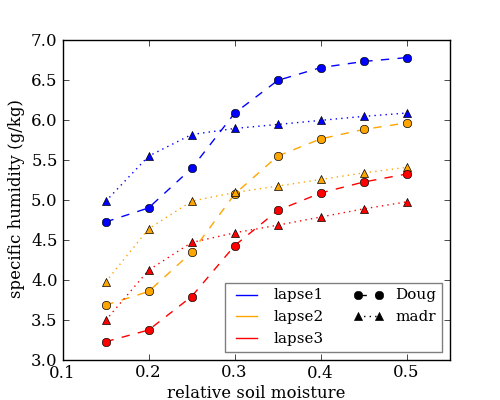
\includegraphics[width=\textwidth]{ch2-BL/figures/all_afternoon_Q.png}
\caption{}
\end{subfigure}
\caption{Conditions at 3:45 pm in the 1-D model, as a function of soil moisture, for the three free troposphere lapse rates (colors).  (a) Air temperature at 400 m ASL (ground level in ACRR), and (b) specific humidity.  Dashed lines with circles: Douglas fir case.  Dotted lines with triangles: Pacific madrone case.}
\label{fig:BL_345changes}
\end{figure}

%\clearpage

For both the Pacific madrone forest and the Douglas fir forest, drier soil (decreasing $\theta_{rel}$) leads to a warmer and drier boundary layer (increasing $T_a$ and decreasing $Q$).  However, in the Douglas fir case, the increase in $T_a$ and decrease in $Q$ begin when the soil is wetter ($\theta_{rel} \le 0.3$; Figures \ref{fig:BL_1DdiurnalTa} and \ref{fig:BL_1DdiurnalQ}, left columns), while in the Pacific madrone case, the increase in $T_a$ and decrease in $Q$ begin only when soil is drier ($\theta_{rel} \le 0.2$; Figures \ref{fig:BL_1DdiurnalTa} and \ref{fig:BL_1DdiurnalQ}, right columns).  

The differences between the species cases are largest in the afternoon; Figure \ref{fig:BL_345changes} shows $T_a$ and $Q$ at 3:45 pm for the Douglas fir and Pacific madrone cases, as a function of $\theta_{rel}$ and free troposphere conditions.  The differences between the Douglas fir and Pacific madrone cases for both $T_a$ and $Q$ are largest at $\theta_{rel}$ values around 0.2, with the Douglas fir case hotter by 1-1.5 $^\circ$C and drier by $\sim$0.7 g/kg.  A $\theta_{rel}$ value of 0.2-0.25 is typical for the mid- to late-dry-season at the ACRR (Figure \ref{fig:sapflow_met}). Interestingly, at $\theta_{rel}$ values higher than about 0.35, the Douglas fir case is actually cooler and moister; such $\theta_{rel}$ values are typical for the late spring and early summer at the ACRR (Figure \ref{fig:sapflow_met}).

\begin{figure}[here]
\begin{subfigure}{0.5\textwidth}
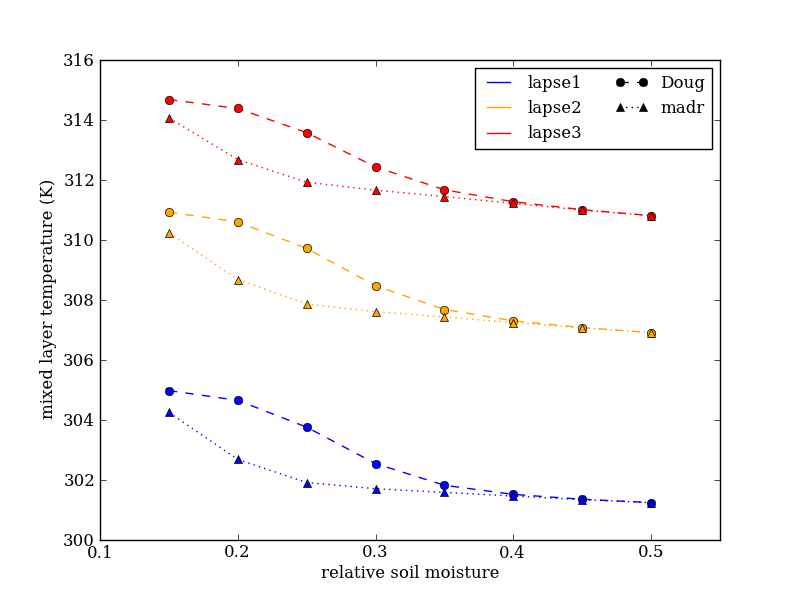
\includegraphics[width=\textwidth]{ch2-BL/figures/theta_afternoon_T.png}
\caption{}
\end{subfigure}
\begin{subfigure}{0.5\textwidth}
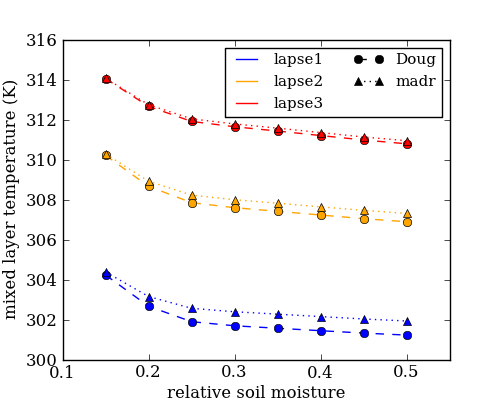
\includegraphics[width=\textwidth]{ch2-BL/figures/VPD_afternoon_T.png}
\caption{}
\end{subfigure}
\caption{Air temperature at 400 m ASL (ground level in ACRR) at 3:45 pm in the 1-D model, as a function of soil moisture, for the three free troposphere lapse rates (colors).  (a) holding $VPD$ parameters constant at Douglas fir values and varying $\theta$ parameters by species, and (b) holding $\theta$ parameters constant at Pacific madrone values and varying $VPD$ parameters by species.}
\label{fig:BL_testVPDtheta}
\end{figure}

The temperature and humidity differences at $\theta_{rel} \le 0.3$ are due largely to Douglas firs' greater stomatal closure with dry soil.  Model tests setting the $VPD$ parameters ($D_o$ and $g_{c,max}$) to the Douglas fir values (Table \ref{tbl:sapflow_mcmc}) and varying the $\theta$ parameters ($\theta_0$ and $\beta$) by species give a Douglas fir - Pacific madrone temperature difference of 1.5-2$^\circ$C at $\theta_{rel} = 0.2$ (Figure \ref{fig:BL_testVPDtheta}(a)), while tests setting the $\theta$ parameters to the Pacific madrone values and varying the $VPD$ parameters by species give a temperature difference of \textless 0.5$^\circ$C at $\theta_{rel} = 0.2$ (Figure \ref{fig:BL_testVPDtheta}(b)).  Thus, in dry soil, the Douglas fir $VPD$ response does little to moderate the temperature differences caused by Douglas fir stomatal closure at low $\theta_{rel}$.  However, in wet soils ($\theta_{rel}$ \textless $0.3$), and particularly in cool free troposphere conditions, the greater Douglas fir stomatal conductance at low $VPD$ cools the boundary layer (Figure \ref{fig:BL_testVPDtheta}(b)), while soil moisture plays little role (Figure \ref{fig:BL_testVPDtheta}(a)).

%- fraction of moisture from land surface vs. from free troposphere, for different soil moisture / lapse rate / species conditions

\subsection{Regional climate model}

\begin{figure}[here]
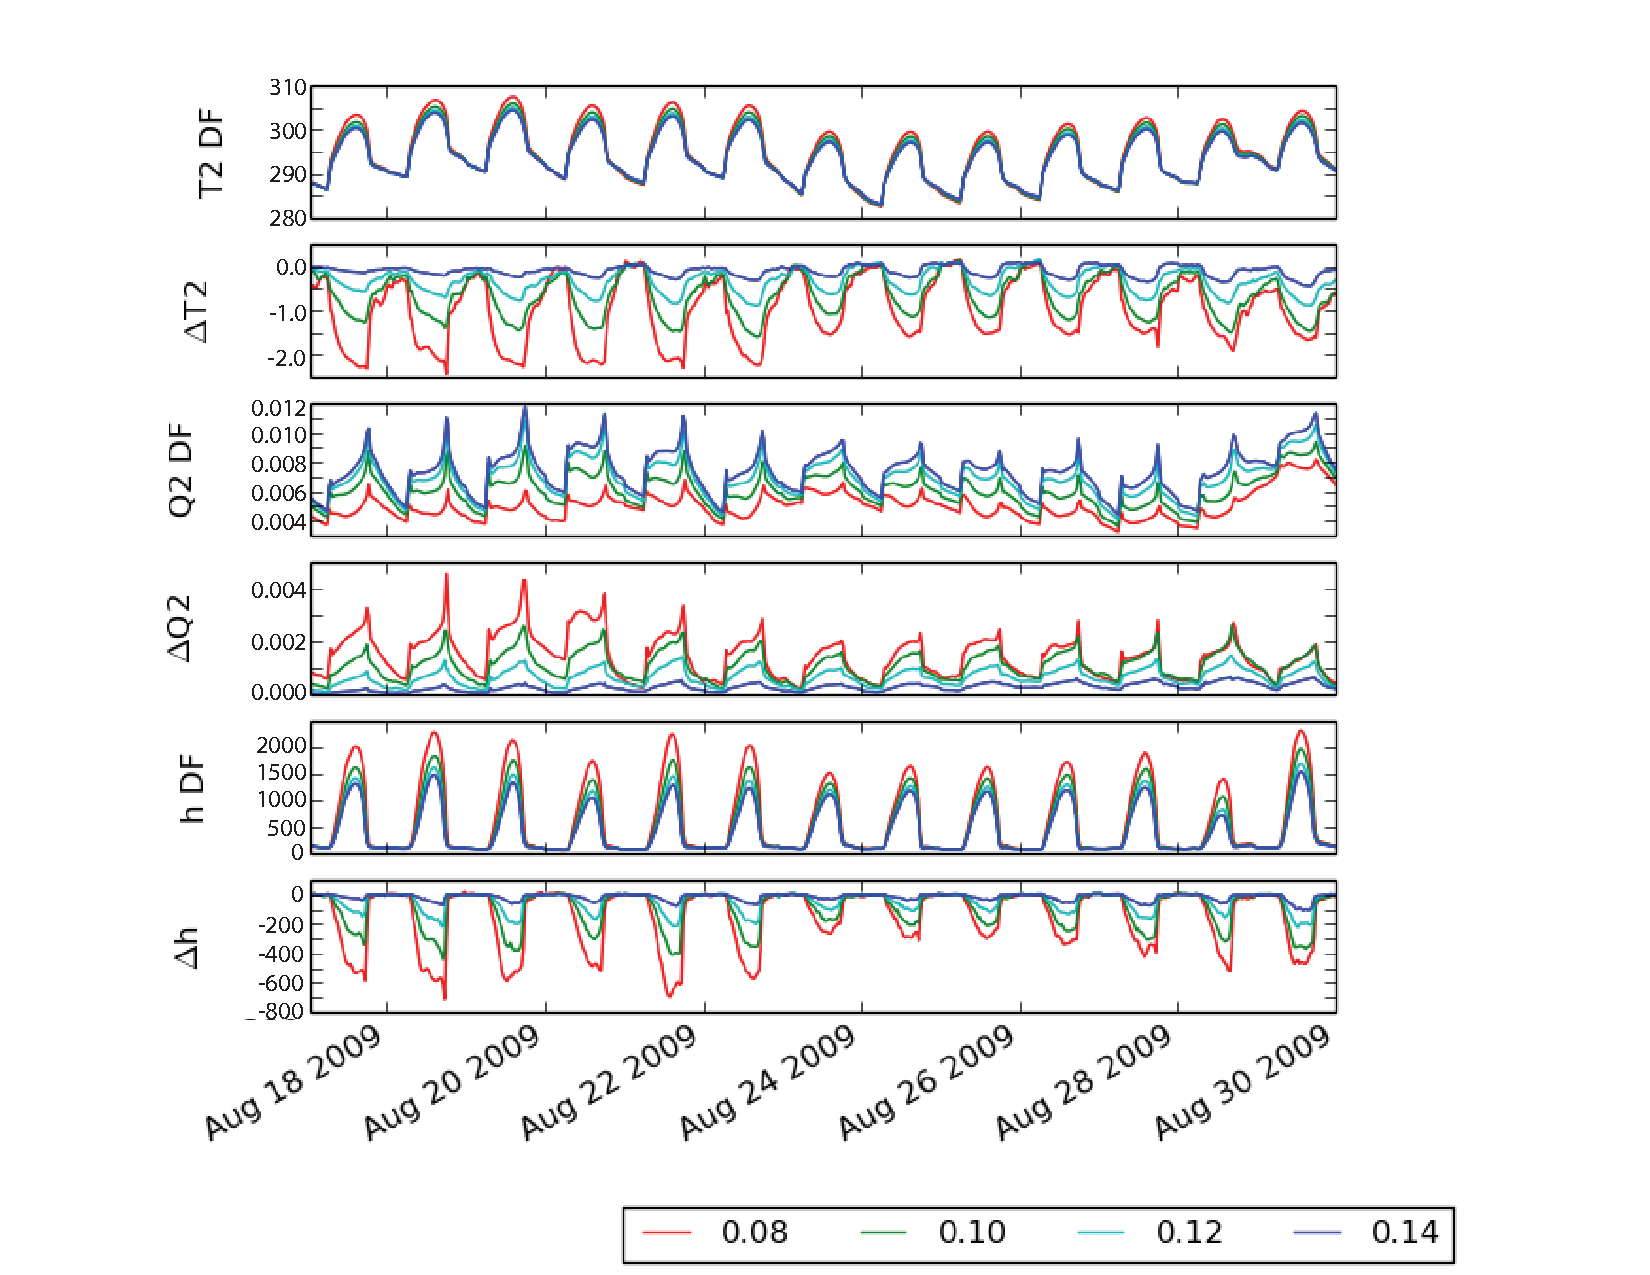
\includegraphics[width=\textwidth]{ch2-BL/figures/T_Q_h_d02.pdf}
\caption{Time series of near-surface conditions in the WRF tests, averaged over the test region, for a range of $\theta_{vol}$ values (colors).  Top panel: air temperature (K) at 2 m above ground level for the all-Douglas-fir case.  Second panel: difference in 2 m air temperature between the all-Pacific-madrone case and the all-Douglas-fir case.  Third panel: specific humidity ($q$, kg/kg) at 2 m above ground, for the all-Douglas-fir case.  Fourth panel: difference in 2 m $q$ between the all-Pacific-madrone case and the all-Douglas-fir case.  Fifth panel: boundary layer height in the all-Douglas-fir case.  Sixth panel: difference in boundary layer height between the all-Pacific-madrone case and the all-Douglas-fir case.}
\label{fig:BL_WRFtseries}
\end{figure}

Figure \ref{fig:BL_WRFtseries} shows the time series of atmospheric conditions averaged over the test region in the Douglas fir case (panels 1, 3, and 5) and the difference between the Pacific madrone and Douglas fir case (panels 2, 4, and 6).  In the Douglas fir case, drier soils lead to a hotter (panel 1 of Figure \ref{fig:BL_WRFtseries}), drier (panel 3), and deeper (panel 5) boundary layer than do wet soils.  For soil moisture $\le$ 0.12 m$^3$/m$^3$ ($\theta_{rel} \le 0.27$), the boundary layer over the madrone forest is cooler (panel 2), moister (panel 4), and shallower (panel 6) than that over the Douglas fir forest; the differences are negligible for soil moisture of 0.14 m$^3$/m$^3$ ($\theta_{rel} = 0.32$).  The differences between the species cases increase with drier soil: the greatest differences occur when soil moisture is 0.08 m$^3$/m$^3$, with 2 m air temperature in the madrone case cooler by 1.5-2.5$^\circ$C, 2 m humidity greater by 1-3 g/kg, and boundary layer depth shallower by 200-500 m, averaged over the test region.

\begin{figure}[here]
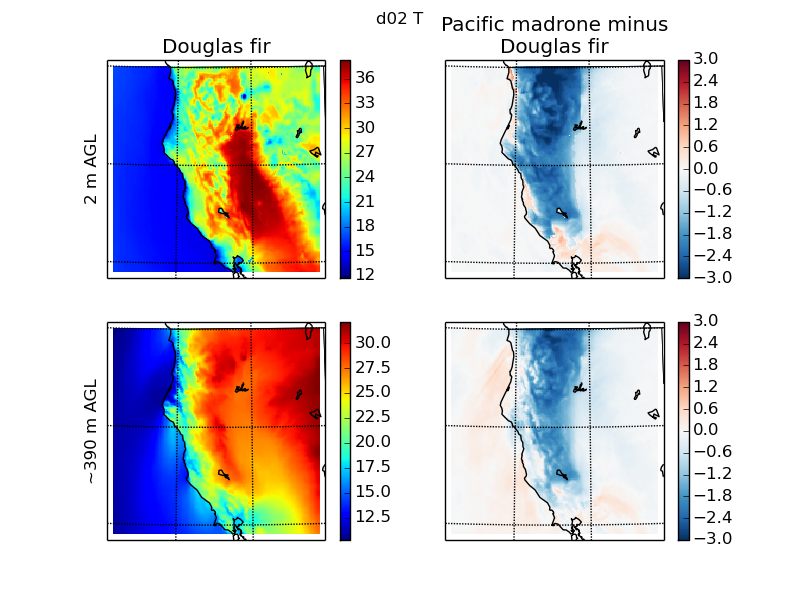
\includegraphics[width=1\textwidth]{ch2-BL/figures/T_d02_s0pt08.png}
\caption{Left column: temperature ($^\circ$C) in domain d02 for the Douglas fir case.  Right column: temperature difference between the Pacific madrone case and the Douglas fir case.  Top row: 2 m above ground level (AGL).  Bottom row: model level at $\sim$390 m AGL (380-395 m for the test region).}
\label{fig:BL_WRFmapT}
\end{figure}

\begin{figure}[here]
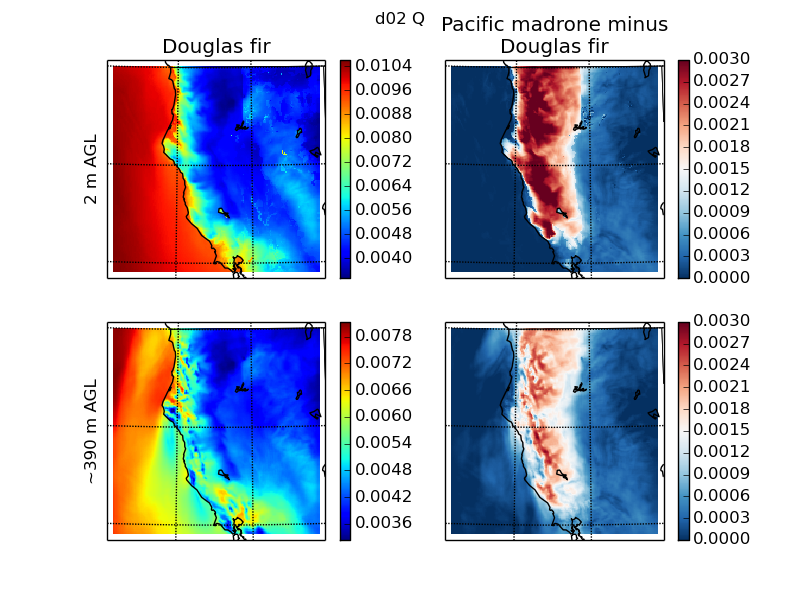
\includegraphics[width=1\textwidth]{ch2-BL/figures/Q_d02_s0pt08.png}
\caption{Left column: specific humidity (kg/kg) in domain d02 for the Douglas fir case.  Right column: specific humidity difference between the Pacific madrone case and the Douglas fir case.  Top row: 2 m AGL.  Bottom row: model level at $\sim$390 m AGL (380-395 m for the test region).}
\label{fig:BL_WRFmapQ}
\end{figure}

\begin{figure}[here]
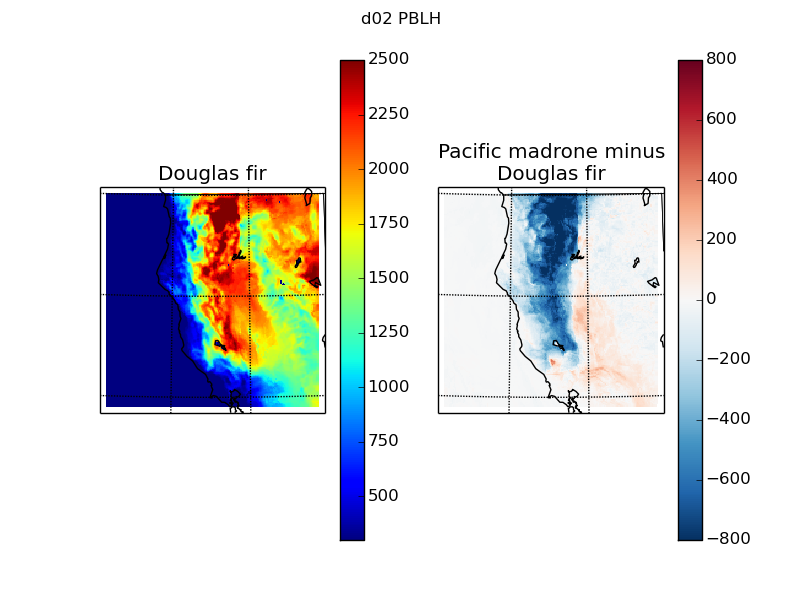
\includegraphics[width=1\textwidth]{ch2-BL/figures/PBLH_d02_s0pt08.png}
\caption{Left column: boundary layer height (m) in domain d02 for the Douglas fir case.  Right column: boundary layer height difference (m) between the Pacific madrone case and the Douglas fir case.}
\label{fig:BL_WRFmapPBLH}
\end{figure}

The differences in temperature and humidity persist from 2 m AGL (Figures \ref{fig:BL_WRFmapT} and \ref{fig:BL_WRFmapQ}, top rows) through to the mixed layer at $\sim$390 m AGL (Figures \ref{fig:BL_WRFmapT} and \ref{fig:BL_WRFmapQ}, bottom rows). The species differences are smaller at 390 m AGL than at 2 m AGL: the madrone case is cooler than the Douglas fir case by up to $\sim$2.5$^\circ$C at 2 m AGL and by up to $\sim$1.5$^\circ$C at 390 m AGL; humidity in the madrone case is greater than in the Douglas fir case by 2-3 g/kg at 2 m AGL and by 1.5-2.5 g/kg at 390 m AGL.

The changes in 390 m AGL temperature and humidity and in boundary layer depth are greatest inland, where the convective boundary layer is fully developed.  The boundary layer in the control Douglas fir case is shallow near the coast but deepens inland (Figure \ref{fig:BL_WRFmapPBLH}, left panel), as expected from previous analytical and numerical studies [\cite{garratt1990internal}].  Because the boundary layer is shallow in this zone, the differences in surface energy balance between the species cases may not be fully communicated to an altitude of 390 m AGL.  The deeper boundary layer inland means that the air at 390 m AGL is part of the mixed layer that communicates rapidly with the surface; thus, the changes in temperature and humidity in the madrone case affect the air at 390 m AGL over inland but not coastal regions.


